% Template for Cogsci submission with R Markdown

% Stuff changed from original Markdown PLOS Template
\documentclass[10pt, letterpaper]{article}

\usepackage{cogsci}
\usepackage{pslatex}
\usepackage{float}
\usepackage{caption}

% amsmath package, useful for mathematical formulas
\usepackage{amsmath}

% amssymb package, useful for mathematical symbols
\usepackage{amssymb}

% hyperref package, useful for hyperlinks
\usepackage{hyperref}

% graphicx package, useful for including eps and pdf graphics
% include graphics with the command \includegraphics
\usepackage{graphicx}

% Sweave(-like)
\usepackage{fancyvrb}
\DefineVerbatimEnvironment{Sinput}{Verbatim}{fontshape=sl}
\DefineVerbatimEnvironment{Soutput}{Verbatim}{}
\DefineVerbatimEnvironment{Scode}{Verbatim}{fontshape=sl}
\newenvironment{Schunk}{}{}
\DefineVerbatimEnvironment{Code}{Verbatim}{}
\DefineVerbatimEnvironment{CodeInput}{Verbatim}{fontshape=sl}
\DefineVerbatimEnvironment{CodeOutput}{Verbatim}{}
\newenvironment{CodeChunk}{}{}

% cite package, to clean up citations in the main text. Do not remove.
\usepackage{cite}

\usepackage{color}

% Use doublespacing - comment out for single spacing
%\usepackage{setspace}
%\doublespacing


% % Text layout
% \topmargin 0.0cm
% \oddsidemargin 0.5cm
% \evensidemargin 0.5cm
% \textwidth 16cm
% \textheight 21cm

\title{Parents Calibrate Speech to Children's Vocabulary Knowledge}


\author{Ashley Leung, Alexandra Tunkel, and Daniel Yurovsky \\
        \texttt{\{ashleyleung, aetunkel, yurovsky\}@uchicago.edu} \\
       Department of Psychology \\ University of Chicago}

\begin{document}

\maketitle

\begin{abstract}
Almost all children acquire language, yet the rates of development
differ drastically across individuals. Previous research suggests that
these differences may arise partially from disparities in parental
input, a finding that has been the foundation for quantity-based
intervention programs. However, language development is not simply
absorbing input- language is social in nature. The communicative intent
and interactive nature of language must not be ignored when considering
how parental input influences children's language development. Indeed,
studies have shown that parental responsiveness shapes young children's
language learning. Parental sensitivity (to children's knowledge,
intent, etc.) may thus be a better predictor of children's language
development than mere quantity of speech. The present study examined
whether parents calibrate speech to their children's knowledge in an
interactive game. Our results show that parents modify their language
according to beliefs about their children's vocabulary knowledge, using
longer sentences when describing unfamiliar objects, and shorter
sentences for familiar objects.

\textbf{Keywords:}
parent-child interaction; language development; communication
\end{abstract}

\section{Introduction}\label{introduction}

Children learn language at astonishing rates, acquiring thousands of
words by the time they are toddlers. How do children learn so many words
even before they know how to dress themselves? One account for
children's rapid language acquisition is statistical learning. Young
children can attend to the distributional structure of language,
learning to discriminate words and identify word order from speech
streams (J. R. Saffran, 2003; J. R. Saffran, Aslin, \& Newport, 1996).
Statistical learning can be a powerful tool for early language learning,
and showcases the ability that children have to harvest information from
their surroundings. However, children's language environments may also
play a role in supporting language development.

The way we speak to children often differs from the way we speak to
adults. Child-directed speech (CDS) exists across cultures, and is
characterized by higher pitches and exaggerated enunciations (Cooper \&
Aslin, 1990; Grieser \& Kuhl, 1988). Not only do children prefer CDS
over adult-directed speech (ADS), CDS is also more helpful for language
learning than overheard ADS (Shneidman, Arroyo, Levine, \&
Goldin-Meadow, 2013). One reason why CDS may facilitate language
development is that its structural qualities make speech segmentation
and word learning easier (Thiessen, Hill, \& Saffran, 2005; Yurovsky,
Yu, \& Smith, 2012). Parents also show sensitivity towards children's
development, such that they use simpler and more redundant language when
talking to toddlers, and more complex syntactic structures when speaking
with school-age children (Snow, 1972). Children's language environments
are uniquely suited for their abilities, and these environments change
across development.

Why do parents modify the way they speak according to their children?
One possible explanation is that parents are actively teaching their
children. Indeed, some have posited that CDS is an ostensive cue for
social learning, and that infants are born prepared to attend to these
cues (Csibra \& Gergely, 2009). While it may be true that parents hope
to impart knowledge to their children, we argue that effective
communication is the proximal goal. The field of linguistics has long
established that adults communicate in ways that are efficient. For
example, Grice's (1975) maxim of quantity states that speech should be
as informative as necessary, and no more. Adults are able to adhere to
these maxims, adapting speech according to conversational partners'
knowledge as needed for successful communication (Clark \& Wilkes-gibbs,
1986). We argue that the parent's goal to communicate with their child
drives the change in language use.

As parents seek to communicate with their children, they modify their
language as a means to achieve successful communication. This could be
the reason why parents use simpler language and are more linguistically
aligned with their younger children - they do so in order to communicate
efficiently with their children (Snow, 1972; Yurovsky, Doyle, \& Frank,
2016). Parents are also sensitive to children's vocabulary knowledge,
and the way they refer to objects change markedly depending on whether
they are novel, comprehended, or familiar to their children (Masur,
1997).

\section{General Formatting
Instructions}\label{general-formatting-instructions}

For general information about authoring in markdown, see
\textbf{\href{http://rmarkdown.rstudio.com/authoring_basics.html}{here}.}

For standard spoken papers and standard posters, the entire contribution
(including figures, references, everything) can be no longer than six
pages. For abstract posters, the entire contribution can be no longer
than one page. For symposia, the entire contribution can be no longer
than two pages.

The text of the paper should be formatted in two columns with an overall
width of 7 inches (17.8 cm) and length of 9.25 inches (23.5 cm), with
0.25 inches between the columns. Leave two line spaces between the last
author listed and the text of the paper. The left margin should be 0.75
inches and the top margin should be 1 inch.
\textbf{The right and bottom margins will depend on whether you use
U.S. letter or A4 paper, so you must be sure to measure the width of
the printed text.} Use 10 point Times Roman with 12 point vertical
spacing, unless otherwise specified.

The title should be in 14 point, bold, and centered. The title should be
formatted with initial caps (the first letter of content words
capitalized and the rest lower case). Each author's name should appear
on a separate line, 11 point bold, and centered, with the author's email
address in parentheses. Under each author's name list the author's
affiliation and postal address in ordinary 10 point type.

Indent the first line of each paragraph by 1/8\textasciitilde{}inch
(except for the first paragraph of a new section). Do not add extra
vertical space between paragraphs.

\section{First-Level Headings}\label{first-level-headings}

First level headings should be in 12 point , initial caps, bold and
centered. Leave one line space above the heading and
1/4\textasciitilde{}line space below the heading.

\subsection{Second-Level Headings}\label{second-level-headings}

Second level headings should be 11 point , initial caps, bold, and flush
left. Leave one line space above the heading and 1/4\textasciitilde{}
line space below the heading.

\subsubsection{Third-Level Headings}\label{third-level-headings}

Third-level headings should be 10 point , initial caps, bold, and flush
left. Leave one line space above the heading, but no space after the
heading.

\section{Formalities, Footnotes, and
Floats}\label{formalities-footnotes-and-floats}

For more information on citations in RMarkdown, see
\textbf{\href{http://rmarkdown.rstudio.com/authoring_bibliographies_and_citations.html\#citations}{here}.}

\subsection{Footnotes}\label{footnotes}

Indicate footnotes with a number\footnote{Sample of the first
footnote.} in the text. Place the footnotes in 9 point type at the
bottom of the page on which they appear. Precede the footnote with a
horizontal rule.\footnote{Sample of the second footnote.} You can also
use markdown formatting to include footnotes using this
syntax.\footnote{Sample of a markdown footnote.}

\subsection{Figures}\label{figures}

All artwork must be very dark for purposes of reproduction and should
not be hand drawn. Number figures sequentially, placing the figure
number and caption, in 10 point, after the figure with one line space
above the caption and one line space below it. If necessary, leave extra
white space at the bottom of the page to avoid splitting the figure and
figure caption. You may float figures to the top or bottom of a column,
or set wide figures across both columns.

\subsection{Two-column images}\label{two-column-images}

You can read local images using png package for example and plot it like
a regular plot using grid.raster from the grid package. With this method
you have full control of the size of your image. \textbf{Note: Image
must be in .png file format for the readPNG function to work.}

You might want to display a wide figure across both columns. To do this,
you change the \texttt{fig.env} chunk option to \texttt{figure*}. To
align the image in the center of the page, set \texttt{fig.align} option
to \texttt{center}. To format the width of your caption text, you set
the \texttt{num.cols.cap} option to \texttt{2}.

\begin{CodeChunk}
\begin{figure*}[h]

{\centering 
\includegraphics{figs/2-col-image-1} 

}

\caption[This image spans both columns]{This image spans both columns. And the caption text is limited to 0.8 of the width of the document.}\label{fig:2-col-image}
\end{figure*}
\end{CodeChunk}

\subsection{One-column images}\label{one-column-images}

Single column is the default option, but if you want set it explicitly,
set \texttt{fig.env} to \texttt{figure}. Notice that the
\texttt{num.cols} option for the caption width is set to \texttt{1}.

\begin{CodeChunk}
\begin{figure}[H]

{\centering 
\includegraphics{figs/image-1} 

}

\caption[One column image]{One column image.}\label{fig:image}
\end{figure}
\end{CodeChunk}

\subsection{R Plots}\label{r-plots}

You can use R chunks directly to plot graphs. And you can use latex
floats in the fig.pos chunk option to have more control over the
location of your plot on the page. For more information on latex
placement specifiers see
\textbf{\href{https://en.wikibooks.org/wiki/LaTeX/Floats,_Figures_and_Captions}{here}}

\begin{CodeChunk}
\begin{figure}[H]

{\centering 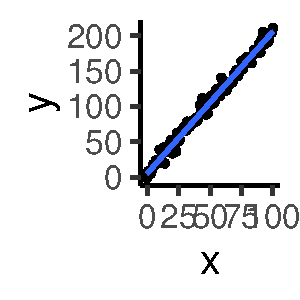
\includegraphics{figs/plot-1} 

}

\caption[R plot]{R plot}\label{fig:plot}
\end{figure}
\end{CodeChunk}

\subsection{Tables}\label{tables}

Number tables consecutively; place the table number and title (in 10
point) above the table with one line space above the caption and one
line space below it, as in Table 1. You may float tables to the top or
bottom of a column, set wide tables across both columns.

You can use the xtable function in the xtable package.

\begin{table}[H]
\centering
\begin{tabular}{rrrrr}
  \hline
 & Estimate & Std. Error & t value & Pr($>$$|$t$|$) \\ 
  \hline
(Intercept) & -0.15 & 0.10 & -1.5 & 0.14 \\ 
  x & 2.05 & 0.10 & 20.8 & 0.00 \\ 
   \hline
\end{tabular}
\caption{This table prints across one column.} 
\end{table}

\section{Acknowledgements}\label{acknowledgements}

Place acknowledgments (including funding information) in a section at
the end of the paper.

\section{References}\label{references}

\setlength{\parindent}{-0.1in} \setlength{\leftskip}{0.125in} \noindent

\hypertarget{refs}{}
\hypertarget{ref-Clark1986}{}
Clark, H. H., \& Wilkes-gibbs, D. (1986). Referring as a collaborative
process, Cognition, 22 (1986) l-39 1, \emph{22}, 1--39.

\hypertarget{ref-Cooper1990}{}
Cooper, R. P., \& Aslin, R. N. (1990). Preference for Infant-Directed
Speech in the First Month after Birth. \emph{Child Development},
\emph{61}(5), 1584--1595.

\hypertarget{ref-Csibra2009}{}
Csibra, G., \& Gergely, G. (2009). Natural pedagogy. \emph{Trends in
Cognitive Sciences}, \emph{13}(4), 148--153.
\url{http://doi.org/10.1016/j.tics.2009.01.005}

\hypertarget{ref-Grieser1988}{}
Grieser, D. A. L., \& Kuhl, P. K. (1988). Maternal Speech to Infants in
a Tonal Language: Support for Universal Prosodic Features in Motherese.
\emph{Developmental Psychology}.
\url{http://doi.org/10.1037/0012-1649.24.1.14}

\hypertarget{ref-Masur1997}{}
Masur, E. F. (1997). Maternal labelling of novel and familiar objects:
implications for children's development of lexical constraints.
\emph{Journal of Child Language}, \emph{24}, 427--439. Retrieved from
\url{https://www.cambridge.org/core/terms.}

\hypertarget{ref-Saffran2003}{}
Saffran, J. R. (2003). Statistical Language Learning: Mechanisms and
Constraints. \emph{Current Directions in Psychological Science},
\emph{12}(4), 110--114. \url{http://doi.org/10.1111/1467-8721.01243}

\hypertarget{ref-Saffran1996}{}
Saffran, J. R., Aslin, R. N., \& Newport, E. L. (1996). Statistical
Learning by 8-Month-Old Infants. \emph{Science}, \emph{274}(5294),
1926--1928. \url{http://doi.org/10.1126/science.274.5294.1926}

\hypertarget{ref-Shneidman2013}{}
Shneidman, L. A., Arroyo, M. E., Levine, S. C., \& Goldin-Meadow, S.
(2013). What counts as effective input for word learning? \emph{Journal
of Child Language}, \emph{40}(3), 672--686.
\url{http://doi.org/10.1017/S0305000912000141}

\hypertarget{ref-Snow1972}{}
Snow, C. E. (1972). Mothers' Speech to Children Learning Language.
\emph{Child Development}, \emph{43}(2), 549--565.

\hypertarget{ref-Thiessen2005}{}
Thiessen, E. D., Hill, E. A., \& Saffran, J. R. (2005). Infant-Directed
Speech Facilitates Word Segmentation. \emph{Infancy}, \emph{7}(1),
53--71. \url{http://doi.org/10.1207/s15327078in0701_5}

\hypertarget{ref-Yurovsky2016}{}
Yurovsky, D., Doyle, G., \& Frank, M. C. (2016). Linguistic input is
tuned to children's developmental level. In \emph{Proceedings of the
38th annual meeting of the cognitive science society} (pp. 2094--2098).

\hypertarget{ref-Yurovsky2012}{}
Yurovsky, D., Yu, C., \& Smith, L. B. (2012). Statistical speech
segmentation and word learning in parallel: Scaffolding from
child-directed speech. \emph{Frontiers in Psychology}, \emph{3}.
\url{http://doi.org/10.3389/fpsyg.2012.00374}

\end{document}
